% !TEX root = ../main.tex
\section{Agentomkostninger (Agency Costs)}\label{thr:agency-costs}

\paragraph{Definisjon.} \emph{Agentomkostninger} (agency costs) er den samlede verditapen som oppstår fordi en agent ikke handler fullt ut i prinsipalens interesse. Jensen \& Meckling (1976) dekomponerer kostnaden i tre komponenter: \textbf{monitoring costs} (prinsipalens utgift til overvåking), \textbf{bonding costs} (agentens utgift til troverdighetssignaler) og \textbf{residual loss} (det gjenværende effektivitetstapet etter at monitoring og bonding er gjort optimalt). [SLIDE]

\subsection*{Forklaring}

I en \thref{principal-agent}{prinsipal--agent}-relasjon skaper agenten verdi for prinsipalen, men har egne preferanser (innsatsaversjon, risikoaversjon, perks, statusbygging). Når informasjon er asymmetrisk, kan ikke prinsipalen presist observere agentens handlinger. Resultatet er at \emph{first-best} (full informasjon, ingen interessekonflikt) ikke er nåbar -- og forskjellen mellom first-best og det realiserte utfallet er den totale agentomkostningen. [SLIDE/BOK]

Den klassiske dekomponeringen lyder:
\[
  \text{Agency costs} \;=\; \underbrace{M}_{\text{monitoring}} \;+\; \underbrace{B}_{\text{bonding}} \;+\; \underbrace{RL}_{\text{residual loss}}.
\]
Prinsipalen velger $M$ og agenten velger $B$ for å minimere \emph{summen} -- ikke for å fjerne $RL$ helt. Det er dyrt å overvåke perfekt, og det er dyrt å binde seg perfekt; en optimal kontrakt aksepterer at en del av tapet blir liggende igjen. [BOK]

\subsubsection*{1. Monitoring costs}
Prinsipalens utgifter til å observere, måle og kontrollere agentens adferd: revisjon, regnskapssystemer, KPI-er, internkontroll, audit committees, eksterne revisorer, rapporteringskrav, IT-overvåking. Eksempel: et sentralisert ERP-system som logger alle innkjøp er monitoring-investering. [SLIDE]

\subsubsection*{2. Bonding costs}
Agentens egne utgifter til å \emph{signalere} eller \emph{garantere} at hun ikke vil utnytte informasjonsovertaket. Eksempler: ledelsesopsjoner som binder lederen til selskapets aksjekurs, restriktive covenants i låneavtaler, deferred compensation, profesjonell sertifisering, frivillige rapporteringsstandarder, og medarbeidereierskap. Bonding er agentens måte å si: ``hvis jeg svikter, taper jeg også''. [SLIDE/BOK]

\subsubsection*{3. Residual loss}
Det gjenværende effektivitetstapet -- forskjellen mellom realisert utfall og first-best -- som blir igjen \emph{etter} at monitoring og bonding er drevet til optimum. Residual loss er ikke et tegn på dårlig kontraktsdesign; det er bevis på at \thref{costless-contracting}{costless contracting} ikke gjelder, og at kompromisset mellom kontroll og kostnad er nådd. [SLIDE]

\subsection*{Tallregnskap fra slide 31 (kap.\ 10)}

\begin{center}
\begin{tabular}{@{}lr@{}}
\toprule
\textbf{Post} & \textbf{Verdi} \\
\midrule
Bruttoverdi av handel & 2\,500 \\
Contracting / out-of-pocket & $-$800 \\
Monitoring costs & $-$400 \\
Bonding costs & $-$400 \\
Residual loss & $-$100 \\
\midrule
Netto verdi $S'$ & 1\,600 \\
\bottomrule
\end{tabular}
\end{center}
\textit{Eksempel fra slide: agentomkostningene reduserer verdien av en handel som i first-best ville vært 2\,500 til 1\,600. Hvis monitoring + bonding hadde vært dyrere enn residual loss de fjerner, ville handelen blitt uattraktiv. [SLIDE]}

\subsection*{Kjerneforutsetninger}
\begin{itemize}
\item \textbf{Asymmetrisk informasjon.} Hvis prinsipalen kunne observere agenten kostnadsfritt, var monitoring overflødig.
\item \textbf{Interessekonflikt.} Hvis agentens nyttefunksjon var sammenfallende med prinsipalens, ville bonding ikke gi mening.
\item \textbf{Risikoaversjon hos agenten} (typisk). Sterkere risikoadeling overfor agent øker bonding-effekten, men også residual loss via redusert insentivstyrke.
\item \textbf{Kontrakter er ufullstendige} ($\Rightarrow$ \thref{costly-contracting}{costly contracting}). Agentomkostninger er en direkte konsekvens av at perfekte tilstandskontrakter ikke kan skrives.
\item \textbf{Begrenset rasjonalitet og positive transaksjonskostnader} (Coase, Williamson).
\end{itemize}

\subsection*{Muligheter (hva forklarer/løser teorien?)}
\begin{itemize}
\item Forklarer \emph{hvorfor virksomheter eksisterer i en bestemt form} -- eierstruktur, kapitalstruktur, kompensasjonsdesign og konsernarkitektur er svar på agentomkostninger.
\item Forklarer hvorfor enkelte transaksjoner organiseres internt (vertikal integrasjon) i stedet for via marked: hvis agentomkostninger ved hierarki $<$ transaksjonskostnader ved marked, internalises transaksjonen.
\item Begrunnelse for sammensetningen av insentivlønn, opsjoner, eierandeler og restriktive covenants -- alt sammen bonding-mekanismer.
\item Begrunnelse for revisor, styreverv, audit committees, intern revisjon -- monitoring-mekanismer.
\item Forutsetning for hele \emph{organizational architecture}-tenkningen: arkitekturen i S1, S2, S3 finnes for å minimere agentomkostninger.
\end{itemize}

\subsection*{Begrensninger og kritikk}
\begin{itemize}
\item \textbf{Måleproblem:} Agentomkostninger er sjelden direkte målbare -- bare residual loss observeres indirekte. Hvor mye som er ``optimalt'' er en teoretisk konstruksjon.
\item \textbf{Risiko for over-monitoring:} For mye overvåking kan ødelegge tillit, intrinsisk motivasjon og kreativitet (crowding-out). Slidene viser ikke dette eksplisitt, men er sentralt i moderne kritikk (Frey, 1997).
\item \textbf{Bonding er ikke gratis for prinsipalen heller:} Insentivlønn og opsjoner overfører risiko til agenten, som krever risikopremie -- jf.\ \thref{informativeness-principle}{informativeness-prinsippet}.
\item \textbf{Opportunistisk re-tolkning:} Ledere kan begrunne nesten enhver utgift som ``monitoring'' eller ``bonding''; konseptene er normative og kan misbrukes.
\item \textbf{Statisk modell:} Klassisk Jensen \& Meckling antar engangsoppsett. Implicit / reputational contracts og gjentatte spill (jf.\ \thref{game-theory}{spilteori}) reduserer agentomkostninger over tid uten å øke $M$ eller $B$.
\item \textbf{Multi-prinsipalproblemer:} Når en agent tjener flere prinsipaler (CEO i børsnotert selskap har aksjonærer, kreditorer, ansatte), blir dekomponeringen mer komplisert.
\end{itemize}

\subsection*{Modell / illustrasjon}

\begin{figure}[H]
\centering
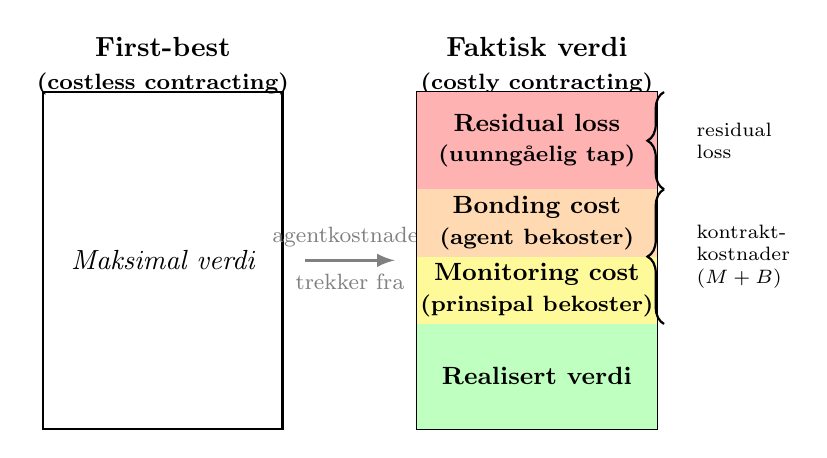
\begin{tikzpicture}[>=latex, scale=0.95, every node/.style={font=\small}]
  % First-best baseline
  \draw[thick] (0,0) rectangle (3.2,4.5);
  \node[font=\bfseries, align=center] at (1.6,4.85) {First-best\\\footnotesize (costless contracting)};
  \node[font=\itshape] at (1.6,2.25) {Maksimal verdi};
  % Pil mellom
  \draw[->, very thick, gray] (3.5,2.25) -- (4.7,2.25);
  \node[gray, font=\footnotesize, above] at (4.1,2.3) {agentkostnader};
  \node[gray, font=\footnotesize, below] at (4.1,2.2) {trekker fra};
  % Andre kolonne: stablet dekomp
  \draw[thick] (5,0) rectangle (8.2,4.5);
  \node[font=\bfseries, align=center] at (6.6,4.85) {Faktisk verdi\\\footnotesize (costly contracting)};
  % Residual loss (øverst)
  \fill[red!30] (5,3.2) rectangle (8.2,4.5);
  \node[font=\bfseries\small, align=center] at (6.6,3.85)
    {Residual loss\\ \footnotesize (uunngåelig tap)};
  % Bonding
  \fill[orange!30] (5,2.3) rectangle (8.2,3.2);
  \node[font=\bfseries\small, align=center] at (6.6,2.75)
    {Bonding cost\\ \footnotesize (agent bekoster)};
  % Monitoring
  \fill[yellow!40] (5,1.4) rectangle (8.2,2.3);
  \node[font=\bfseries\small, align=center] at (6.6,1.85)
    {Monitoring cost\\ \footnotesize (prinsipal bekoster)};
  % Realiserte verdi
  \fill[green!25] (5,0) rectangle (8.2,1.4);
  \node[font=\bfseries\small, align=center] at (6.6,0.7)
    {Realisert verdi};
  % Klammer
  \draw[decorate, decoration={brace, amplitude=6pt}, thick]
    (8.3,3.2) -- (8.3,4.5)
    node[midway, right=8pt, font=\scriptsize, align=left] {residual\\ loss};
  \draw[decorate, decoration={brace, amplitude=6pt}, thick]
    (8.3,1.4) -- (8.3,3.2)
    node[midway, right=8pt, font=\scriptsize, align=left] {kontrakt-\\ kostnader\\ ($M+B$)};
\end{tikzpicture}
\caption{\textbf{Agency cost-dekomponering} (Jensen \& Meckling 1976; BSZ kap.\ 10, slide 7). Avviket fra first-best splittes i tre: \emph{Monitoring costs} (M, prinsipalens overvåking), \emph{Bonding costs} (B, agentens forpliktelser/risiko-bæring) og \emph{Residual loss} (uunngåelig tap pga.\ ikke alle insentivkonflikter kan utelukkes kostnadseffektivt). Total agency cost = $M + B + \text{residual loss}$. [SLIDE]}
\end{figure}

\subsection*{Eksempler}
\begin{itemize}
\item \textbf{Equinor / aksjonærer:} Norsk stat (\textasciitilde 67\%) krever omfattende monitoring via styre, riksrevisjon og åpenhetsregler. CEO-bonding skjer via aksjebasert kompensasjon. Residual loss er likevel synlig: politiske beslutninger om f.eks.\ Trans-Adriatic Pipeline eller fornybarsatsninger som ikke maksimerer NPV. [EKS]
\item \textbf{Mærsk McKinney Møller-fonden:} A.P. Møller-Mærsk har en stiftelseskontrollert eierstruktur som reduserer agentomkostninger ved at langsiktige eiere overvåker direkte; men residual loss kommer i form av begrenset adgang til ekstern kapital ved store satsinger som Power-to-X. [CASE]
\item \textbf{Lehman Brothers (2008):} Eksempel på utilstrekkelig monitoring (svake risikomodeller, manglende styrekontroll) kombinert med pervers bonding (bonus knyttet til kortsiktig P\&L). Residual loss = konkursen selv. [EKS]
\item \textbf{IKEA:} Familiekontrollert via Stichting INGKA Foundation reduserer monitoring-behovet og lar selskapet investere langsiktig. Bonding skjer gjennom kulturelle normer (``IKEA-vägen'') og medarbeideropplæring i Älmhult. [EKS]
\end{itemize}

\subsection*{Kobling til søyle og andre teorier}
Agency costs spenner over alle tre søyler: \SOne\ (hvem som får beslutningsrett bestemmer hvor stor residual loss kan bli), \STwo\ (monitoring \emph{er} prestasjonsmåling), \SThree\ (bonding \emph{er} insentivdesign). Relaterte: \thref{principal-agent}{Principal--agent}, \thref{moral-hazard}{Moral hazard}, \thref{adverse-selection}{Adverse selection}, \thref{costly-contracting}{Costly contracting}, \thref{costless-contracting}{Costless contracting}, \thref{specific-vs-general-knowledge}{Spesifik vs.\ generell viden}, \thref{organizational-architecture}{Organizational architecture}, \thref{informativeness-principle}{Informativeness-prinsippet}.

\paragraph{Brukt i spørsmål:} Q04, Q05, Q06, Q09, Q10, Q11, Q12, Q14.
